\documentclass[a4paper,oneside,12pt]{report}

\usepackage[utf8]{inputenc}
\usepackage[french]{babel}
\usepackage{graphicx}
\usepackage{hyperref}
\usepackage{setspace}
\usepackage{color}
\usepackage{listings}
\usepackage{fancyhdr}
\usepackage{array}


\newcommand{\atemplate}{template}
\newcommand{\atemplates}{templates}

\newcommand{\apartial}{partial}
\newcommand{\apartials}{partials}

\newcommand{\aplugin}{plugin}
\newcommand{\aplugins}{plugins}

\newcommand{\awidget}{widget}
\newcommand{\awidgets}{widgets}

\newcommand{\afm}{framework}
\newcommand{\afms}{frameworks}

\newcommand{\aminidev}{minidev}
\newcommand{\aminidevs}{minidevs}

\newcommand{\abug}{bug}
\newcommand{\abugs}{bugs}

\newcommand{\anewsletter}{newsletter}

\newcommand{\alotun}{lot~1}
\newcommand{\alotdeux}{lot~2}

\newcommand{\asladmin}{slAdminPlugin}
\newcommand{\asismo}{Sismo}
\newcommand{\asf}{Symfony}
\newcommand{\asvn}{Subversion}
\newcommand{\asl}{Sensio~Labs}
\newcommand{\aintranet}{Intranet}
\newcommand{\aey}{Eyrolles}
\newcommand{\ayml}{YML}
\newcommand{\aphp}{PHP}
\newcommand{\alc}{La~Croix}



\title{Stage d'assistant ingénieur chez \asl}
\author{Jérémy Subtil}

\hypersetup{
	pdftitle     = {TN09 - Rapport de stage},
	pdfauthor    = {Jérémy Subtil},
	pdfsubject   = {Stage d'assistant ingénieur chez \asl},
	pdfkeywords  = {site web, \aphp, \afm, \asf, programmation orientée objet, \amvc, base de données, \aorm, \adoctrine}
}


\renewcommand{\lstlistlistingname}{Table des listings de code}
\lstset{
	language		= PHP,	
	tabsize			= 2,
	frame			= single,
	breaklines		= true, 
	basicstyle		= \scriptsize\ttfamily,
	keywordstyle	= \bfseries,
	numbers         = left,
	stepnumber      = 5,
	numberstyle		= \tiny,
	firstnumber		= 1,
	captionpos		= b
}

\lstdefinelanguage{YML}{}


\lhead{\begin{small}\nouppercase{\leftmark}\end{small}}
\rhead{\begin{small}\nouppercase{\rightmark}\end{small}}


\graphicspath{{figs/}}


\begin{document}

\section*{Remerciements}

Merci à \ahugon\ de m'avoir donné ma chance pour participer à l'aventure \asl.

Merci à toute l'équipe du pôle développement pour leurs conseils, leur \acoaching\ et leurs légendaires fortunes.

Plus généralement, merci à l'ensemble du personnel de \asensio\ pour leur accueil chaleureux, leur bonne humeur et toute l'expérience qu'ils ont pu m'apporter.

Merci à mon suiveur de stage à l'\autc, \asuiveur, pour ses conseils pratiques.

Merci à \apotencier\ et aux contributeurs de \asf\ pour leur investissement dans l'écosystème du logiciel libre.

Enfin, merci à \asarah\ pour son soutien et sa patience.

\newpage

\tableofcontents
\listoffigures
\listoftables
\lstlistoflistings
\newpage

\begin{abstract}

Résumé

\end{abstract}
\newpage

\pagestyle{fancy}

\chapter{Présentation de l'entreprise}

\section{L'entreprise \asensio}

La société \asensio\ a été créée en 1988 par les deux co-fondateurs \apotencier\ et \apascal. Dès ses premiers mois, elle s'est très vite orientée vers les technologies de l'\ainternet. Elle s'inscrit alors comme une véritable agence web interactive, proposant à ses clients un savoir-faire dans tous les métiers du web : développement, expertise technique, \awm, communication et \awd. Aujourd'hui, elle est basée dans la ville de Clichy, située près de Paris.

En 2007, \asensio\ s'est rapprochée d'\aextreme\footnote{À l'occasion du 29\ieme\ Grand Prix des \aagencesannee\ en 2009, \aextreme\ s'est vu décerner le prix du groupe de communication indépendant de l'année.}, un grand groupe in\-dé\-pen\-dant de communication globale\footnote{publicité, marketing, services, web, \textit{packaging}, design, \textit{corporate}\dots}. Cette démarche commerciale, et non capitalistique, distingue bien les deux entités en deux sociétés à part entière. Elle a pour origine un désir des deux parties : d'un côté \aextreme\ souhaitait se rapprocher d'une agence web, et de l'autre, \asensio\ ressentait le besoin d'acquérir de meilleures compétences dans le domaine de la communication.

L'association de \asensio\ et d'\aextreme\ a donné naissance à trois entités commerciales, ou \abusfull :

\begin{description}
	\item[\asl] s'occupe de la partie développement web ;
	\item[\aes] gère tout l'aspect \awm\ et communication ;
	\item[\aesm] propose à ses clients des plans média destinés à doper leur trafic et leurs ventes.
\end{description}

La force de \asensio\ réside donc dans le fait de pouvoir faire travailler ensemble des personnes aux profils de natures très différentes, et cela afin de répondre au mieux aux attentes de ses clients.

Rentable dès ses débuts, \asensio\ dégage un chiffre d'affaires de 6~millions d'euros pour l'année~2009, d'après les estimations actuelles.


\section{La \abufull\ \asl}

Chez \asensio, j'ai travaillé dans la \abufull\ \asl. Dirigée par \apotencier, son cœur de métier est de développer des applications web pour les grands comptes. En effet, ses principaux clients sont Peugeot, EDF, l'Office de Tourisme et des Congrès de Paris, Infogreffe, Evian\dots

Par ailleurs, \asl\ est le créateur d'un outil de travail connaissant aujourd'hui un succès international formidable : le \afm\ \aphp\ \asf\ décrit en section~\ref{section:outils_sf}. Celui-ci apporte à l'entreprise une visibilité grandissante associée à une image de marque. 

\asl\ est constitué de trois pôles aux ambitions différentes :

\begin{description}
	\item[le pôle projet] est composé de chefs de projets, dont le but est de s'occuper de toute la partie communication avec le client, de faire l'intermédiaire entre les différents acteurs techniques d'un projet, de rédiger son cahier des charges, de planifier le temps et les ressources qui lui sont affectés ;
	\item[le pôle production] est composé d'intégrateurs, qui ont pour objectif de transformer les maquettes de sites, réalisées par les créateurs d'\aes, en pages web statiques compatibles avec un certain nombre de navigateurs du marché ;
	\item[le pôle développement] se compose d'une équipe de développeurs, dont le but est de rendre dynamiques les pages web produites par le pôle production, en se chargeant de l'implémentation de leur logique.
\end{description}

Dans le cadre de mon stage, j'ai travaillé au pôle développement en tant que développeur.

Il faut noter que certains projets, concernant des sites web évènementiels ou promotionnels par exemple, sont orchestrés par les chefs de projets d'\aes\ et non pas par ceux du pôle projet de \asl. Toutefois, les réalisations techniques sont bien issues des pôles production et développement de ce dernier.


\section{Mon choix de \asl}

Au cours de mon année de licence à l'université d'\abrookes\ en Angleterre en 2007, j'ai eu à réaliser un projet individuel et conséquent de développement logiciel. J'ai alors choisi de réaliser une application web expérimentale à mi-chemin entre un \acms\footnote{Un \acms\ (\acmsfull), ou système de gestion de contenu, est une famille de logiciels destinés à la conception et à la mise à jour dynamique de site web ou d'application multimédia.~\cite{cms}} et un réseau social\footnote{Un réseau social est un ensemble d'entités sociales, telles que des individus ou des organisations sociales, reliées entre elles par des liens créés lors d'interactions sociales.~\cite{reseausocial}}. Pour cela, j'ai choisi de développer avec les technologies \aphp\ et \asf. Comme l'utilisation de l'outil issu de \asl\ m'avait beaucoup plu, j'ai tout de suite pensé à postuler dans cette entreprise pour mon stage d'assistant ingénieur. Il s'est avéré que ma connaissance préalable de \asf\ m'a été extrêmement utile pour m'immerger rapidement dans ma mission de stage.

Au-delà de l'enjeu technologique, j'ai été vivement attiré par le fait que \asl, en distribuant son outil sous licence libre\footnote{Une licence libre est une licence s'appliquant à une œuvre d'esprit par laquelle l'auteur concède tout ou une partie des droits que lui confère le droit d'auteur.~\cite{licencelibre}}, est acteur majeur de l'\aos\footnote{La désignation \aos\ s'applique aux logiciels donc la licence respecte des critères précisément établis par l'\aosinitiative, c'est-à-dire la possibilité de libre redistribution, d'accès au code source et de travaux dérivés.~\cite{os}}. En effet, l'écosystème du logiciel libre\footnote{Un logiciel libre est un logiciel dont l'utilisation, l'étude, la modification, la duplication et la diffusion sont universellement autorisées sans contrepartie.~\cite{logiciellibre}} est un domaine qui me passionne, dans lequel j'aimerais éventuellement exercer mon futur métier d'ingénieur. J'ai alors pensé qu'ajouter un tel stage à mon parcours professionnel serait une excellente piste pour m'engager dans cette voie.

Ainsi, travailler chez \asl\ a bien été pour moi le fruit d'un réel désir, et non pas d'un choix par défaut.

\chapter{Stage}

\section{Déroulement du stage} % 2 pages

TODO


\section{Outils utilisés dans l'entreprise}

Cette section présente une liste non exhaustive des outils que j'ai pu utiliser au cours de mon stage.

\subsection{Le langage \aphp}

\aphp\footnote{\url{http://www.php.net}} est le langage de programmation utilisé chez \asl. C'est un langage de script libre principalement utilisé pour produire des pages web dynamiques : le code \aphp\ est intégré dans un document \ahtml\ puis interprété par le serveur web doté d'un module \aphp. Le langage peut également être utilisé via un interpréteur lancé via la ligne de commande, pour exécuter des programmes localement par exemple.

Sa syntaxe est empruntée aux langages C, Java et Perl, afin de rendre le langage plus facile à apprendre. Depuis la version~5, \aphp\ est capable de produire des programmes à la conception orientée objet.


\subsection{Environnements de développement}

Chez \asl, le choix de l'environnement de développement est donné au développeur. Certains utilisent des éditeurs de texte comme \aultraedit\ ou \avim, d'autres des environnements de développement intégré\footnote{Un environnement de développement intégré (EDI ou IDE en anglais) est un programme regroupant un ensemble d'outils pour le développement de logiciels.~\cite{edi}} tels que \aeclipse\ ou \anetbeans.

Pour ma part, j'ai choisi \anetbeans\footnote{\url{http://www.netbeans.org/}}. En effet, j'étais déjà bien habitué à cet environnement, que j'utilisais pour programmer en \ajava\footnote{J'ai d'ailleurs participé au développement du logiciel \agephi\ (\url{http://www.gephi.org/}) qui repose sur la même base que \anetbeans, appelée \anbp.} Il supporte nativement de nombreux langages de programmation, dont notamment \aphp. Il a pu me fournir, entre autres, les facilités suivantes :

\begin{itemize}
	\item une coloration syntaxique des différents formats de fichier supportés par \asf, tels que \aphp, \ahtml\ ou \ayml ;
	\item une auto-complétion de code adaptée à \asf ;
	\item un support intégré de \asvn\footnote{Cf. section\ref{section:outils_svn}}.
\end{itemize}


\subsection{\avservers}

Chez \asl, il existe une machine relativement puissante qui est divisée en plusieurs machines virtuelles surnommées \avservers. Celles-ci ont l'avantage de pouvoir être facilement dupliquées et reviennent beaucoup moins cher que des machines physiques dédiées à la performance équivalente. 

Un \avserver\ prend ainsi l'apparence d'un serveur \alinux\ classique et indépendant. Chacun appartient à un développeur ou à un chef de projet. Son propriétaire est le seul à pouvoir y accéder et en possède les droits administrateurs : il peut donc y installer tous les outils dont il aurait besoin.

Typiquement, le développeur se sert de son \avserver\ pour afficher les pages web qu'il développe grâce au serveur web et au serveur de base de données qui y sont installés. C'est également par ce biais que les chefs de projets ou les autres développeurs peuvent consulter le fruit de son travail.

Finalement, ce système de \avservers\ est un excellent compromis entre uniformisation des environnements de développement et flexibilité.


\subsection{\asvn}
\label{section:outils_svn}

%svnmerge

TODO


\subsection{\asf}

\asf\ est le \afm\ \aphp\ dont l'initiateur est \apotencier, un des co-fondateurs de \asl. Dans un premier temps conservé en interne dans l'agence, il a finalement été distribué sous licence libre en octobre~2005. Depuis, une véritable communauté internationale s'est formée autour de cet outil. Au delà des qualités techniques intrinsèques de \asf, on peut expliquer ce phénomène par le fait que qu'un effort considérable a été fourni concernant l'écriture de documentation : d'abord rédigée en anglais, elle a ensuite été traduite en plusieurs langues. De plus, plusieurs livres techniques\footnote{Références bibliographiques : \cite{practicalsf} \cite{sfrefguide} \cite{cahierssf} \cite{moresf} \cite{thebook}} ont déjà été publiés, dont la plupart voient leur contenu accessible librement et de façon officielle sur \ainternet.

Les parties suivantes abordent successivement une présentation du concept de \afm, du modèle \amvc, qui est utilisé de façon globale dans \asf, et enfin une énumération des différentes fonctionnalités de \asf.


\subsubsection{Le concept de \afm}

TODO


\subsubsection{Le modèle \amvc}

TODO


\subsubsection{Fonctionnalités de \asf}

TODO


\subsection{\adoctrine}
\label{section:outils_doctrine}

TODO


\subsection{\atrac}
\label{section:outils_trac}

\atrac\footnote{\url{http://trac.edgewall.org/}} est un logiciel libre de gestion de projet, prenant la forme d'une interface web. Il inclut notamment un wiki\footnote{Un wiki est un site web dont les pages sont généralement modifiables par l'ensemble des visiteurs du site. Il permet ainsi l'écriture collaborative de documents.~\cite{wiki}} pour partager du contenu, un système de suivi de tickets\footnote{Un ticket comprend généralement un titre, un contenu, et différents statuts de suivi, comme \og nouveau \fg\ ou \og résolu \fg\ par exemple. Un ticket est souvent utilisé pour représenter un rapport de \abug.}, un explorateur de dépôt \asvn\ et une vue d'historique.

Chez \asl, chaque projet possède son propre \atrac, qui facilite sa gestion et son suivi. Ce dernier est utilisé en tant que moyen de communication privilégié entre développeurs, chefs de projet et clients. Il prend tout son intérêt lors des phases de recette, comme on le verra en section~\ref{section:eyrolles_organisation_recette}.


\subsection{\asismo}
\label{section:sismo}

\asismo\ est une application web développée en interne chez \asl. Elle a été écrite en \aphp\ en utilisant le \afm\ \asf.

C'est un outil d'intégration continue. Ce concept consiste à tester automatiquement l'application tout au long de son développement. Cela permet de prévenir les régressions et de détecter facilement où et quand des erreurs ont été introduites.

En effet, pour chaque projet en cours de développement, \asismo\ surveille constamment si de nouveaux changements ont été introduits sur leur dépôt \asvn\ respectif. À intervalle de temps régulier (de l'ordre de la demi-heure), \asismo\ reconstruit chaque projet ayant fait l'objet de modifications depuis la passe précédente. Les tests qui ont été écrits par les développeurs sont alors lancés.

Si toute la batterie de tests d'un projet a réussi, le nom du projet est affiché en vert dans l'interface de liste des projets\footnote{Cf. figure~\ref{figure:outils_sismo_screenshots_liste}} sur \asismo, ou en rouge sinon. Cette vue est particulièrement utile pour repérer rapidement les projets qui posent potentiellement problème.

Sur la fiche d'un projet\footnote{Cf. figure~\ref{figure:outils_sismo_screenshots_projet}} sont affichés les numéros de révision de son dépôt \asvn. Ici aussi, des codes couleur sont utilisés : une révision est verte pour des tests réussis, rouge pour des tests échoués, et gris quand les tests n'ont pas encore été lancés. Ainsi, les développeurs peuvent facilement situer à quel moment les spécifications des tests n'ont plus été respectées grâce à l'intervalle révision verte - révision rouge indiquée par \asismo.

 % 5 pages

\section{Site web des eaux de javel La Croix}
 % 5 pages

\section{Intranet des maisons d'édition Eyrolles}

\subsection{Contexte et objectifs}

TODO

\subsubsection{Planning initial}

TODO

\subsection{Organisation du travail}

\subsubsection{Phase d'analyse}

TODO

\subsubsection{Phase de développement}

TODO

\subsubsection{Phase de recette}

TODO

\subsubsection{Livraison finale}

TODO

\subsubsection{Planning réel}

TODO

\subsection{Fonctionnalités attendues de l'Intranet}

TODO

\subsection{\asladmin}

La plupart des vues du \alotdeux\ de l'\aintranet\ d'\aey\ sont générées grâce au \aplugin\ \asf\ \asladmin. Il a été développé en interne par \asl\ et est issu de l'abstraction du code d'un précédent projet. Il n'a rien à voir avec la fonctionnalité de génération d'administration intégrée à \asf. C'est encore un \aplugin\ très jeune : \aey\ est le premier projet qui l'utilise.

\begin{table}
	\centering
	\begin{tabular}{|p{3cm}||p{4.5cm}|p{4.5cm}|}
		\hline
		& Génération d'administration & \asladmin\ \tabularnewline
		\hline
		\hline
		Format de configuration & \ayml & code \aphp \tabularnewline
		\hline
		Génération de code & oui & non \tabularnewline
		\hline
		Personnalisation de la logique & surcharge de code généré & surcharge de méthodes d'action de base \tabularnewline
		\hline
		Personnalisation des vues & surcharge de \apartials\ générés & écriture classique de \atemplates \tabularnewline
		\hline
	\end{tabular}
	\caption{Comparaison entre la génération d'administration de \asf\ et \asladmin}
	\label{table:eyrolles_sladmin_sladmin-vs-admin-gen}
\end{table}

Le tableau~\ref{table:eyrolles_sladmin_sladmin-vs-admin-gen} reprend une comparaison rapide des différences entre le moteur de génération d'administration de \asf et \asladmin. Le \aplugin\, tout comme la génération d'administration, permet de ne pas avoir à redévelopper la logique des opérations de base, telles que le listing d'éléments, la pagination et le tri de la liste, ou encore la création, l'édition ou la suppression d'éléments. Sa valeur ajoutée est qu'il apporte plus de flexibilité quant à la personnalisation de la logique et des différentes vues.

Un exemple d'implémentation de module utilisant \asladmin\ sera présenté dans la partie~\ref{section:eyrolles_ref-langues}

\asladmin\ s'articule autour de trois composants majeurs :
\begin{itemize}
	\item une classe \aphp\ de configuration ;
	\item des actions d'administration de base ;
	\item des \awidgets\ pour agencer la vue.
\end{itemize}


\subsubsection{La classe de configuration}

La classe de configuration permet de stocker les différents paramètres qui seront utilisés pour configurer les actions et la vue d'un module.

Une classe de configuration doit satisfaire les conditions suivantes :
\begin{itemize}
	\item elle doit être placée dans le dossier \texttt{lib/config} du module et doit être nommée \texttt{slAdminConfigurationMonNomDeModule} ;
	\item elle doit hériter de la classe abstraite \texttt{slBaseAdminConfiguration} du \aplugin\, qui contient la liste de toutes les options disponibles (cf. Figure~\ref{figure:eyrolles_sladmin_config}) ;
	\item la définition des paramètres personnalisés doit se faire dans la méthode \texttt{configure()} surchargée.
\end{itemize}

\begin{figure}
	\centering
	\includegraphics[scale=0.4]{eyrolles_sladmin_config}
	\caption{Classe de configuration de \asladmin}
	\label{figure:eyrolles_sladmin_config}
\end{figure}


\subsubsection{Actions de base}

\asladmin\ contient deux classes d'actions qui servent de base aux actions des modules gérés.

La première, \texttt{slBaseActions}, hérite de la classe \asf\ \texttt{sfActions}. Elle fournit des méthodes pour gérer les messages de confirmation ou les messages d'erreur, ainsi qu'une méthode de validation de formulaire avancée. La seconde classe, \texttt{slAdminActions}, hérite de \texttt{slBaseActions}. C'est elle qui contient toutes les actions d'administration supportées telles que \texttt{show}, \texttt{list}, \texttt{edit}, \texttt{delete}, \texttt{filter}, \texttt{sort} ou \texttt{batch}.

Ainsi, la classe d'actions d'un module utilisant \asladmin\ doit hériter de la classe \texttt{slAdminActions} au lieu de la classique \texttt{sfActions}. Les méthodes d'action peuvent alors être surchargées si nécessaire.

Ce comportement est décrit dans la Figure~\ref{figure:eyrolles_sladmin_actions}.

\begin{figure}
	\centering
	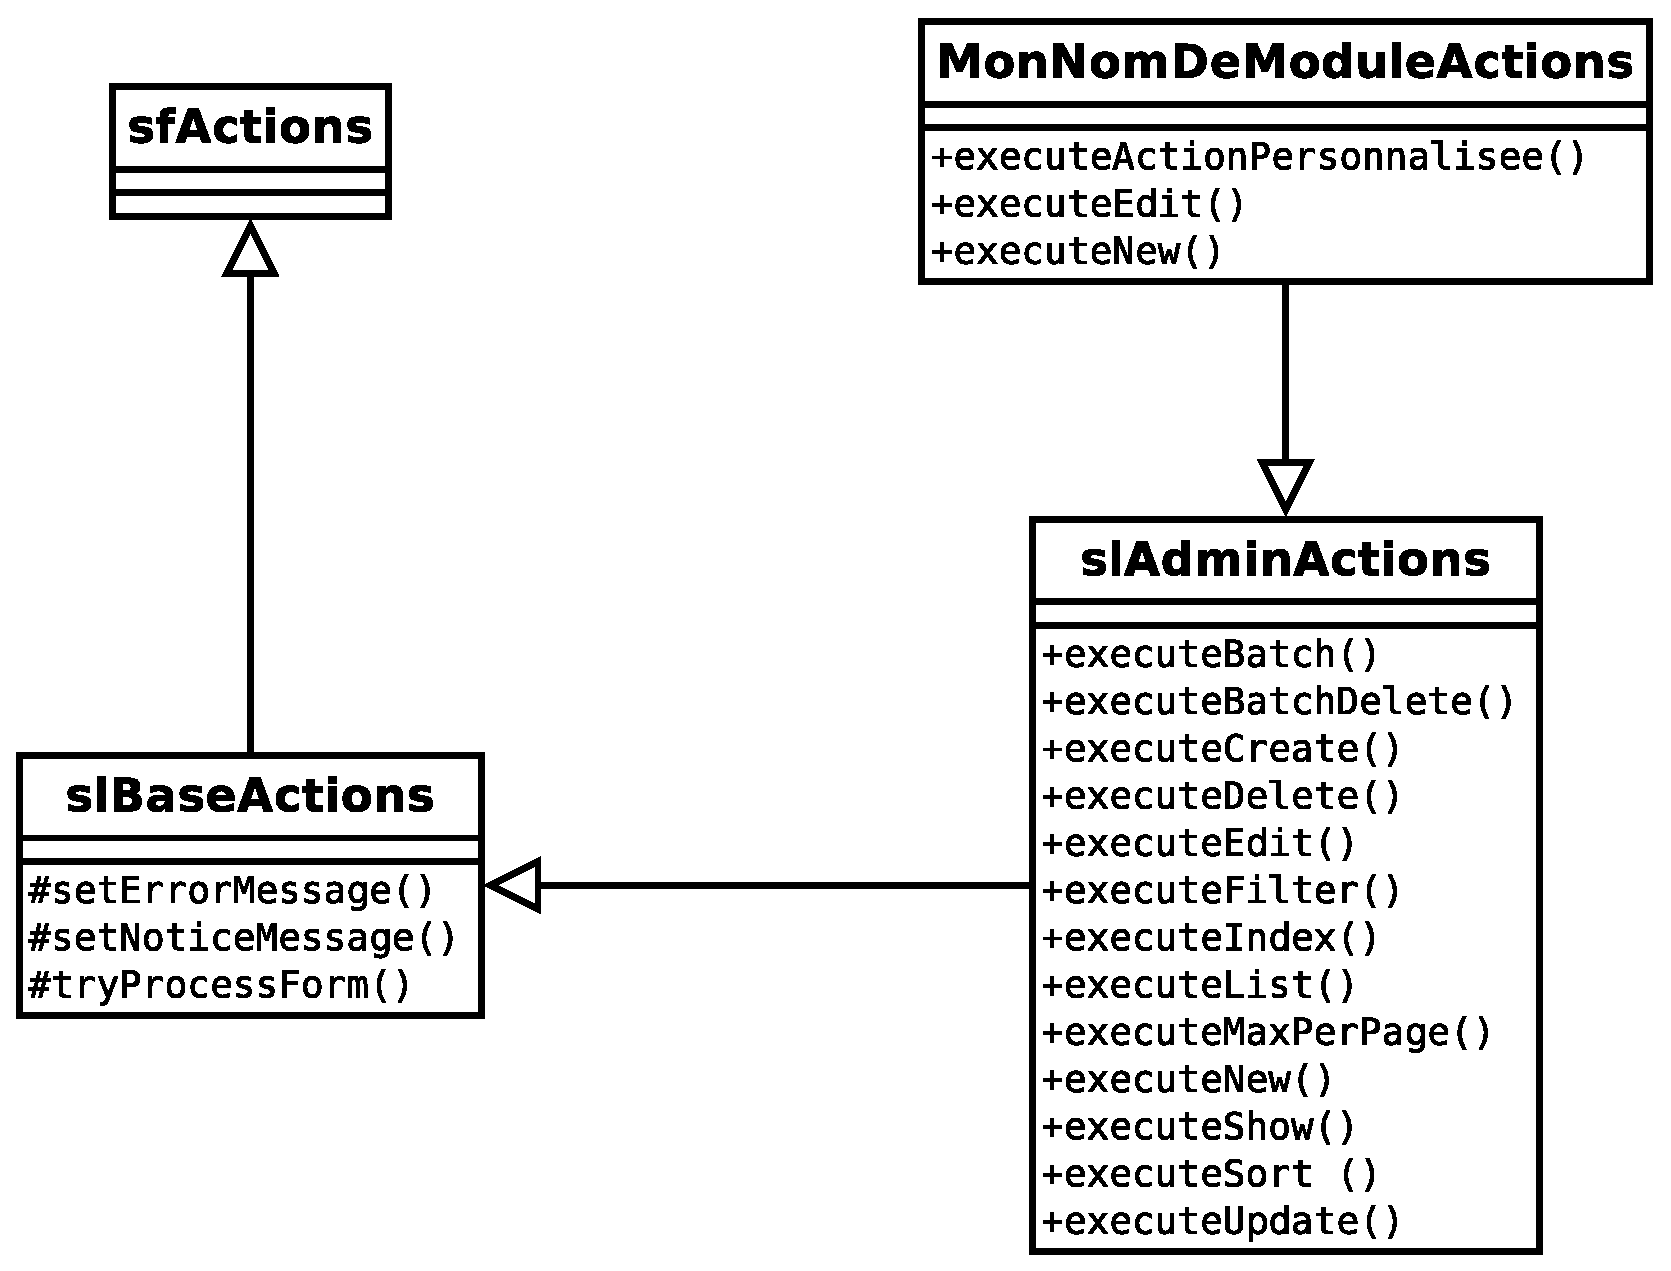
\includegraphics[scale=0.4]{eyrolles_sladmin_actions}
	\caption{Actions de base fournies par \asladmin}
	\label{figure:eyrolles_sladmin_actions}
\end{figure}


\subsubsection{Gestion de la vue}
\label{section:eyrolles_sladmin_view}

À la base, un module utilisant \asladmin\ doit posséder les cinq \atemplates\ suivants :
\begin{description}
	\item[\texttt{listSuccess.php}] -- le \atemplate\ affichant le listing des objets du modèle géré par le module, contenant par exemple les filtres, un tableau d'affichage et un pager ;
	\item[\texttt{listHeader.php}] -- le \apartial\ affichant la ligne de titre du tableau de listing ;
	\item[\texttt{list\_row.php}] -- le \apartial\ affichant une ligne du tableau de listing ;
	\item[\texttt{newSuccess.php}] -- le \atemplate\ affichant le formulaire de création d'objet ;
	\item[\texttt{editSuccess.php}] -- le \atemplate\ affichant le formulaire d'édition d'objet.
\end{description}

Les éléments récurrents de ces vues comme le tableau d'affichage des objets ou le pager sont en réalité des \awidgets, qui sont instanciés dans les actions de base de \asladmin. Le nom des classes de ces \awidgets\ peuvent d'ailleurs être définis dans la classe de configuration du module. Les \awidgets\ peuvent être affichés dans un \atemplate\ comme le montre le Listing~\ref{listing:eyrolles_sladmin_template}.

\lstinputlisting[float, caption={Affichage de \awidgets de \asladmin\ dans un \atemplate}, label={listing:eyrolles_sladmin_template}]{code/eyrolles_sladmin_template.php}


\subsubsection{Surcharge de \asladmin\ pour les besoins de l'application}

Comme la plupart des modules de l'application d'\aey\ utilisent \asladmin, des classes propres au projet ont été insérées entre les classes \texttt{slAdmin} à surcharger habituellement et les classes des différents modules. En fait, ajouter un couche intermédiaire a l'avantage de permettre de personnaliser le comportement de la librairie utilisée tout en la gardant intacte. Il reste alors tout à fait possible de mettre à jour la libraire sans avoir à ré-appliquer les modifications propres au projet. Cette organisation est illustrée dans la Figure~\ref{figure:eyrolles_sladmin_surcharge}.

\begin{figure}
	\centering
	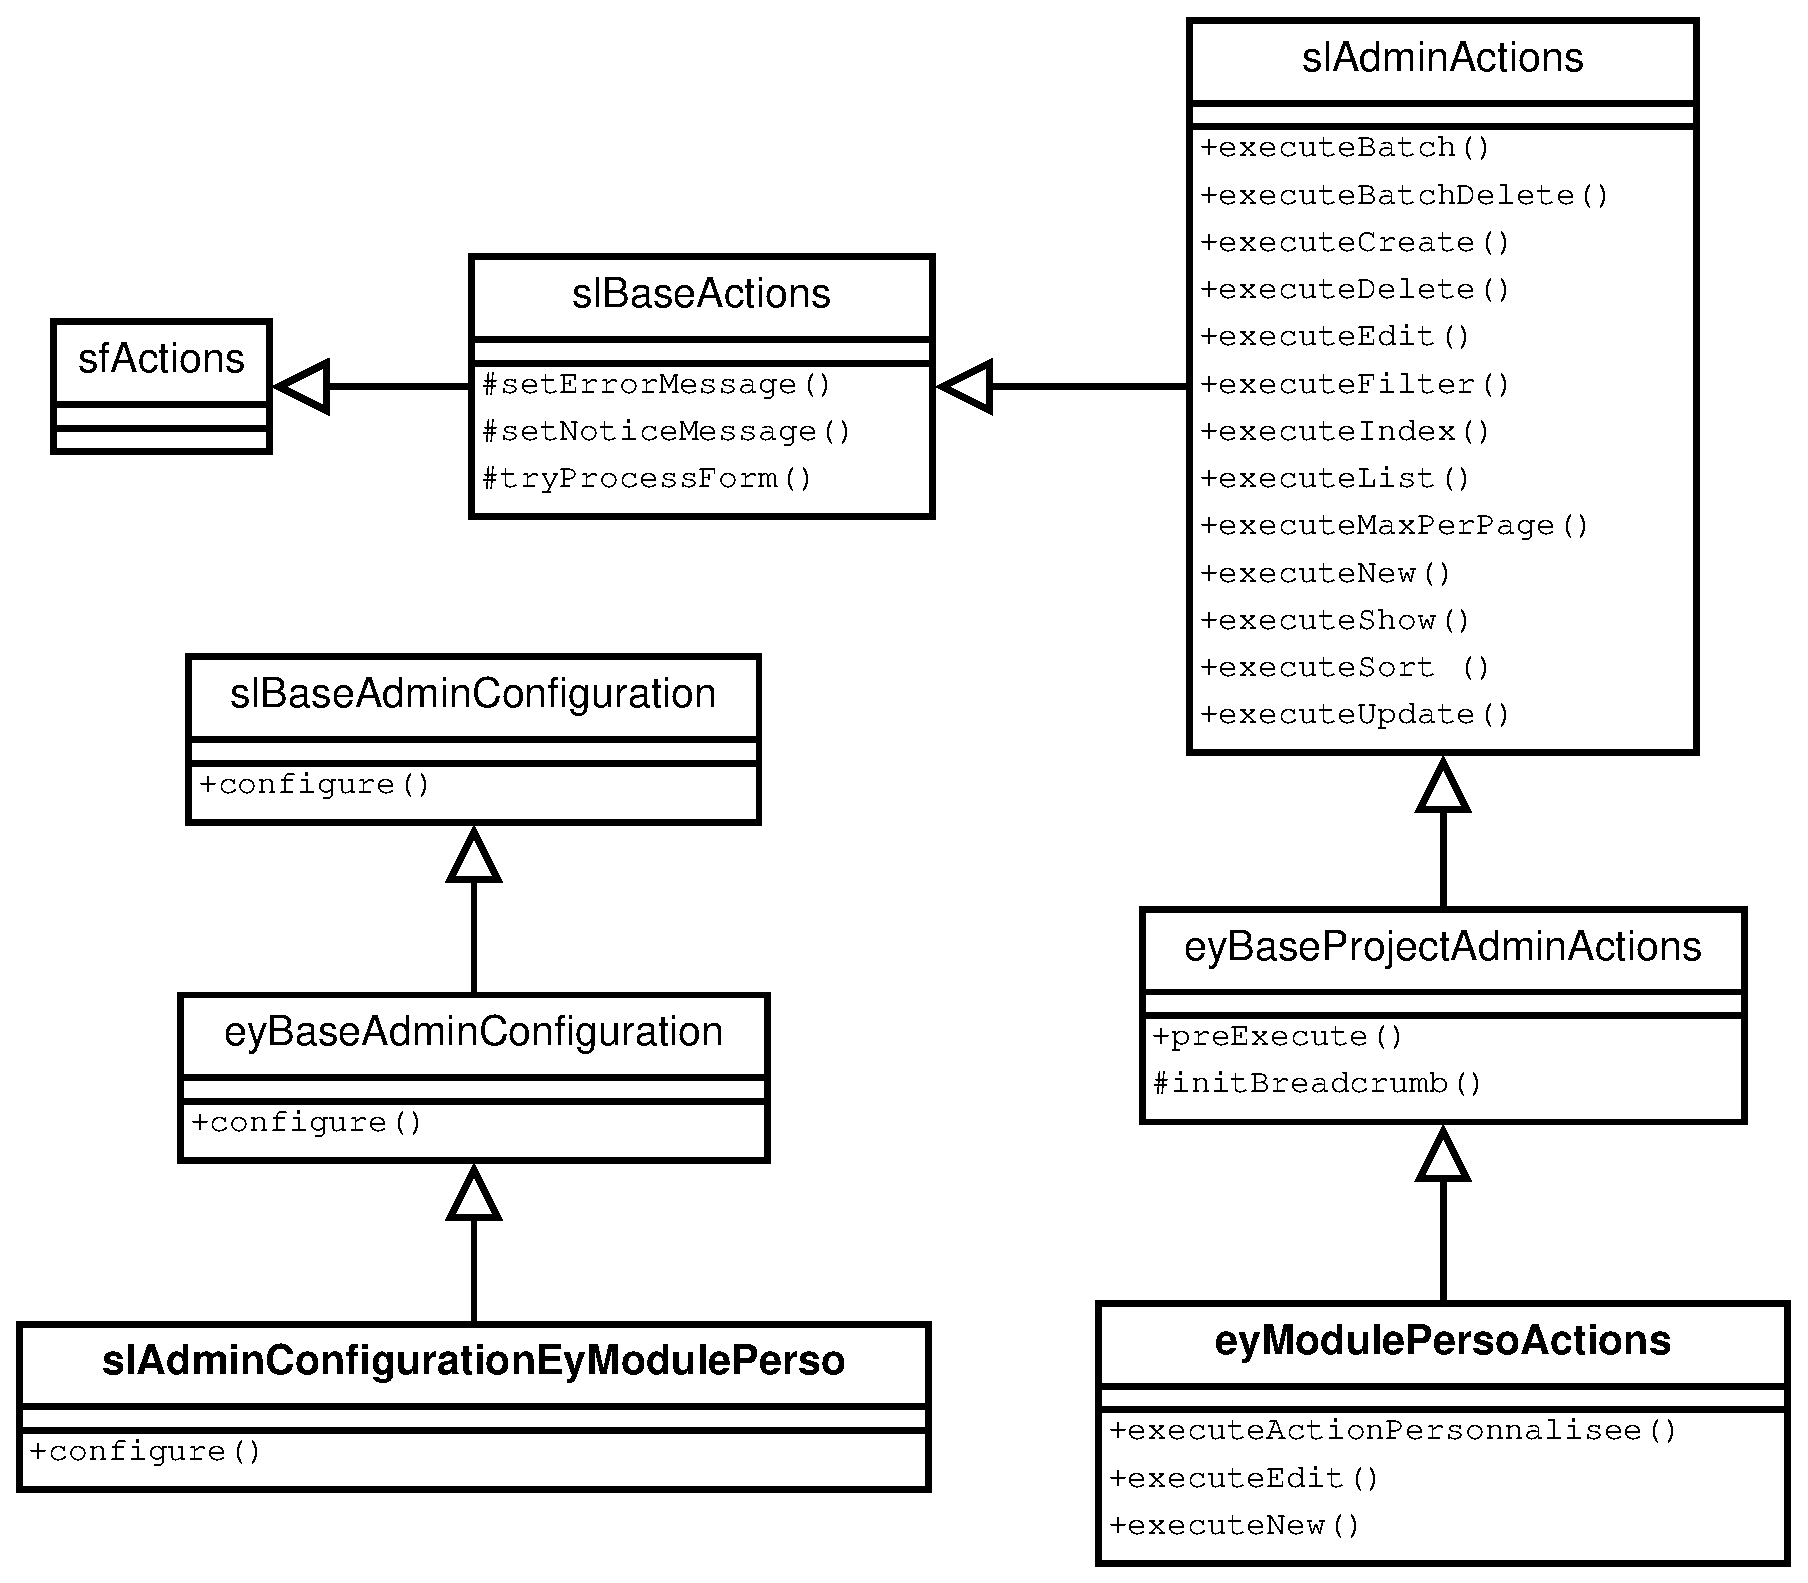
\includegraphics[scale=0.4]{eyrolles_sladmin_surcharge}
	\caption{Surcharge de \asladmin\ dans le cadre du projet \aey}
	\label{figure:eyrolles_sladmin_surcharge}
\end{figure}

Au final, les actions des modules d'\aey\ doivent surcharger la classe \texttt{eyBaseAdminActions}, et les configurations doivent surcharger \texttt{ey\-Base\-Admin\-Configuration}.


\subsection{Un module type : le référentiel des langues}
\label{section:eyrolles_ref-langues}

Le référentiel des langues est l'un des nombreux référentiels administrables de l'application décrits dans la partie~***.

Il est implémenté sous la forme d'un module nommé \texttt{ey\-Referential\-Language} qui utilise \asladmin. En effet, le module doit offrir les fonctionnalités suivantes, qui sont offertes par défaut par le \aplugin\ :
\begin{itemize}
	\item le listings des langues contenues dans la base de données ;
	\item l'ajout et la modification d'une langue ;
	\item la suppression d'une langue.
\end{itemize}

Le module des langues a été choisi pour être décrit car il peut être considéré comme un module qui, tout en restant très simple, est typique de l'application. Les paragraphes suivants rentrent dans le détail de son implémentation, et l'annexe~\ref{section:annexe_eyrolles_ref-langues} regroupe son code et des captures d'écran.


\subsubsection{Arborescence}

L'arborescence de \texttt{eyReferentialLanguage} suit les règles classiques d'organisation d'un module \asf\ et intègre les fichiers nécessaires au bon fonctionnement de \asladmin\ :

\begin{verbatim}
eyReferentialLanguage/
  actions/
    actions.class.php
  lib/
    config/
      slAdminConfigurationEyReferentialLanguage.class
  templates/
    _form.php
    _listTableRow.php
    listSuccess.php
    newSuccess.php
\end{verbatim}

L'organisation des fichiers de \atemplate\ ne suit pas exactement les consignes énoncées en partie~\ref{section:eyrolles_sladmin_view}. En effet, dans la classe de configuration, on a préféré utiliser le nom de \apartial\ \texttt{listTableRow} au lieu de \texttt{list\_row}. Par ailleurs, le \apartial\ \texttt{form} est appelé dans le \atemplate\ \texttt{new}.


\subsubsection{Schéma de la base de données}

Le données du référentiel des langues sont stockées dans une seule table de la base de données nommée \texttt{EyReferentialLanguage}. Elle contient les champs suivants : \texttt{id}, \texttt{label}, \texttt{description} et \texttt{created\_by}. Le champ \texttt{id} est la clé primaire de la table, qui sert à identifier de façon unique chaque langue. Quant au champ \texttt{created\_by}, il est utilisé en tant que clé étrangère vers la table des utilisateurs de l'\aintranet\ \texttt{sfGuardUser} : cette liaison permet de retrouver le créateur de la langue.

Le schéma permettant de créer cette table dans la base de données est repris dans le listing~\ref{listing:eyrolles_ref-langues_schema}. Pour expliciter ce format, un diagramme \auml\ équivalent est proposé en figure~\ref{figure:eyrolles_ref-langues_uml}.

\begin{figure}
	\centering
	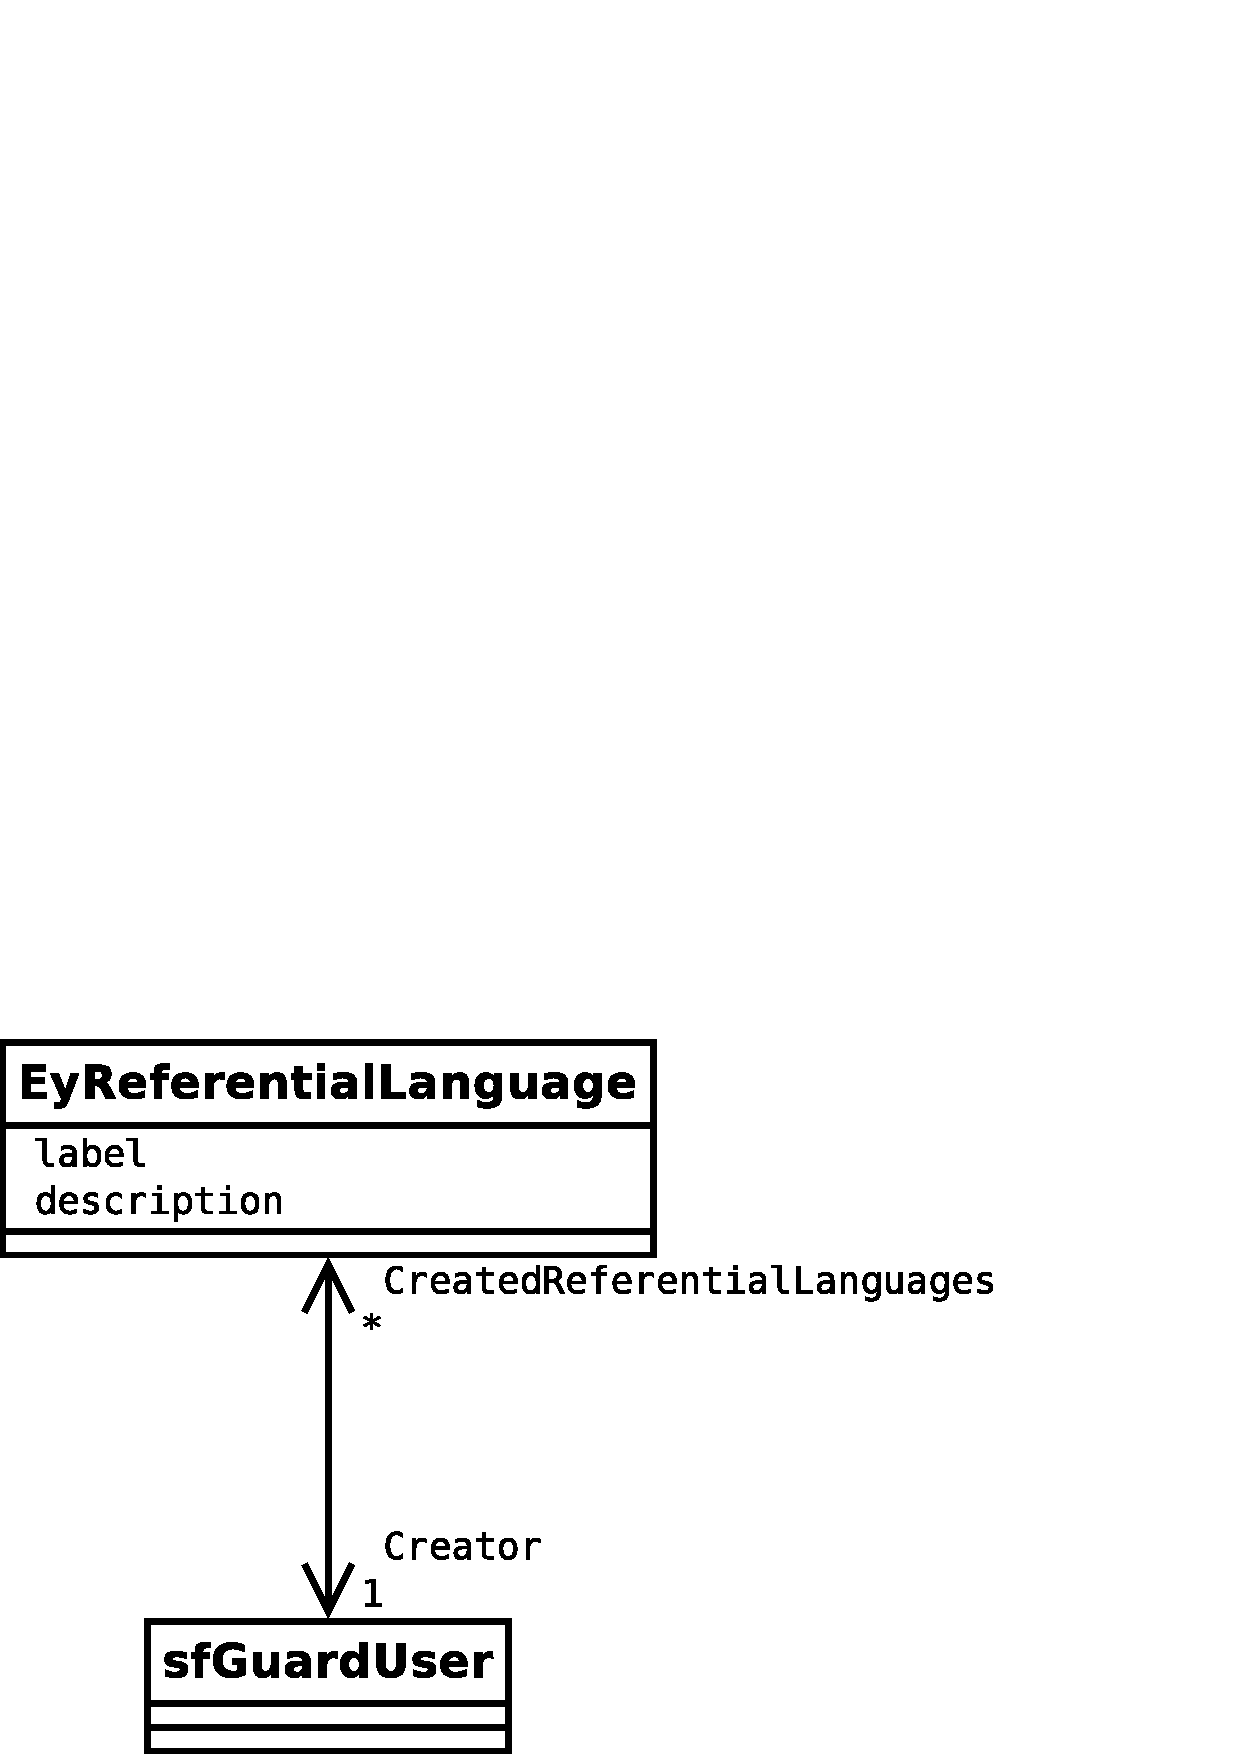
\includegraphics[scale=0.4]{eyrolles_ref-langues_uml}
	\caption{Représentaion \auml\ de la table du référentiel des langues}
	\label{figure:eyrolles_ref-langues_uml}
\end{figure}

On peut noter l'utilisation des mots-clés \texttt{Timestampable} et \texttt{SoftDelete} listés dans la partie \texttt{actAs}. Ce sont ce que l'on appelle des \emph{behaviors} \adoctrine\ : ils peuvent être assimilés à des comportements personnalisés que l'on veut donner à une table.

En effet, le \abehavior\ \texttt{Timestampable} ajoute automatiquement deux champs \texttt{created\_at} et \texttt{updated\_at} dans la table. Respectivement, ils sont remplis automatiquement par une date quand un enregistrement est crée et quand il est mis à jour. En plus de garder une trace du créateur de la langue, \texttt{Timestampable} conservera alors les données temporelles de modification de la table.

Le \abehavior\ \texttt{SoftDelete}, quant à lui, permet de ne jamais supprimer un enregistrement de la base de données. En fait, il ajoute un champ \texttt{deleted\_at} : quand on demande la suppression d'un enregistrement, sa valeur est affectée à la date de la pseudo délétion, sinon sa valeur est nulle. Les différentes requêtes \adoctrine\ écrites par le développeur sont alors automatiquement modifiées pour ignorer les enregistrements qui sont sensés avoir été supprimés. Dans le cas d'\aey, \texttt{SoftDelete} permet d'implémenter nativement l'archivage des données au cas où le client aurait besoin de les restaurer ou d'en générer des statistiques.


\subsubsection{Configuration}

La classe de configuration nécessaire pour \asladmin\ est accessible dans le listing~\ref{listing:eyrolles_ref-langues_config}.

Sans expliciter de façon fastidieuse toutes les options utilisées, elle définit globalement les paramètres suivants :

\begin{itemize}
	\item la classe de modèle à utiliser ;
	\item la requête à utiliser pour récupérer les langues à afficher sur la page de listing (listing~\ref{listing:eyrolles_ref-langues_table}) ;
	\item le champ sur lequel les langues seront triés ;
	\item le nombre maximum de langues affichées sur la page de listing ;
	\item le titre des colonnes du tableau de la page de listing ;
	\item le \apartial\ à utiliser pour afficher une ligne du tableau de listing ;
	\item les classes de formulaire à utiliser.
\end{itemize}


\subsubsection{Routes}

Le fichier de \arouting\ du module est accessible dans le listing~\ref{listing:eyrolles_ref-langues_routing}.

\texttt{eyReferentialLanguage\_batch} est une route classique. La valeur du champ \texttt{url} correspond à l'adresse que l'utilisateur va entrer dans son navigateur pour accéder à l'action \texttt{batch} du module \texttt{eyReferentialLanguage}. L'option \texttt{sf\_method} indique quelle méthode HTTP\footnote{Dans le protocole HTTP, une méthode est une commande spécifiant un type de requête, c'est-à-dire qu'elle demande au serveur d'effectuer une action. \cite{http}} l'utilisateur doit appeler pour que la route soit accessible. Dans le cas de cette route, la méthode est \texttt{POST}, ce qui correspond en fait à la validation d'un formulaire.

La route \texttt{eyReferentialLanguage}, quant à elle, utilise la classe de \arouting\ avancée \texttt{sfDoctrineRouteCollection}. Cette classe intégrée au \afm\ \asf\ a la particularité de générer tout un ensemble routes qui correspondent à des actions de bases. Par exemple, des actions générées sont \texttt{ey\-Re\-fe\-ren\-tial\-Lan\-guage\_\-list}, \texttt{ey\-Re\-fe\-ren\-tial\-Lan\-guage\_\-new}, \texttt{ey\-Re\-fe\-ren\-tial\-Lan\-guage\_\-edit}, correspondent respectivement aux actions \texttt{list}, \texttt{new}, \texttt{edit}, et redirigent respectivement vers le listing des langues, la création d'une langue et son édition.


\subsubsection{Actions}

Les actions du module, situées dans la classe \texttt{ey\-Referential\-Language\-Actions}, reposent sur les actions de base d'\aey\footnote{Voir le listing~\ref{listing:eyrolles_base_actions}}, qui reposent elles-mêmes sur les actions de \asladmin. Elles sont accessibles dans le listing~\ref{listing:eyrolles_ref-langues_actions}.

On remarque que seule l'action \texttt{edit} est redéfinie. En effet, on y ajoute le nom de la langue que l'on est en train d'éditer dans le fil d'Arianne\footnote{Sur un site web, un fil d'Ariane représente l'arborescence des rubriques que le visiteur a traversées depuis la page d'accueil.\cite{breadcrumb}\\Exemple : \texttt{Accueil > Référentiels > Langues > Liste}}. Toutes les autres actions comme \texttt{list} ou \texttt{new} sont en réalité déjà écrites dans les actions de base de \asladmin. Le fait qu'il y ait au final peu de code à écrire est un bon signe : c'est un gain de temps pour le développeur et c'est une bonne opportunité pour ne pas intégrer de \abug. C'est justement ce genre d'avantage qui a incité à utiliser \asladmin\ dans \aey.

Dans les actions de base \texttt{eyBaseAdminActions}, la méthode \texttt{init\-Bread\-crumb()}, qui initialise le fil d'Arianne, est appelée dans la méthode \texttt{pre\-Execute()} : ainsi, le fil d'Arianne est initialisé dans chaque action de l'application \aey. La méthode \texttt{initBreadcrumb()} est surchargée dans \texttt{ey\-Referential\-Language\-Actions} : au mot \textit{Accueil} présent sur toute les pages, on ajoute \textit{Référentiels} puis \textit{Langues}. C'est un bon exemple de la façon typique de surcharger les classes de \asladmin.

Le module du référentiel des langues restant un module très simple, les actions de \asladmin\ n'ont pas trop eu a être surchargées. Dans d'autres modules, qui intègrent une logique métier plus poussée, il est nécessaire d'apporter une surcharge plus importante et d'écrire des actions supplémentaires spécifiques.


\subsubsection{Affichage de la vue}

Les vues, contrairement aux actions, n'ont pas déjà été écrites dans \asladmin\ : c'est au développeur de les implémenter en totalité.

Les \atemplates\ et les \apartials\ utilisés dans le module sont les suivants :

\begin{description}
	\item[\texttt{listSuccess.php}] \atemplate\ du listing des langues (listing~\ref{listing:eyrolles_ref-langues_template-list})
	\item[\texttt{\_listTableRow.php}] \apartial\ des lignes du tableau de listing (listing~\ref{listing:eyrolles_ref-langues_template-row})
	\item[\texttt{newSuccess.php}] \atemplate\ de création d'une langue (listing~\ref{listing:eyrolles_ref-langues_template-new})
	\item[\texttt{\_form.php}] \apartial\ du formulaire de création (listing~\ref{listing:eyrolles_ref-langues_template-form})
\end{description}

Étant donné la quantité de concepts à acquérir pour comprendre les subtilités de la vue, le fonctionnement de ces fichiers de \atemplate\ ne sera pas décrit ici en détail. Pour en savoir plus, il est toutefois possible de se référer à la documentation du \afm\ \asf\cite{thebook}.

Voilà tout de même quelques clés :

\begin{itemize}
	\item les fonctions \texttt{url\_for()} et \texttt{link\_to()} permettent de générer des liens hypertexte à partir des routes passées en paramètre ;
	\item la fonction \texttt{image\_tag()} permet de générer la balise d'une image donnée pour l'afficher dans le navigateur ;
	\item dans \texttt{\_listTableRow.php}, la variable \texttt{\$subject} représente l'instance de l'objet de langue à afficher sur la ligne du tableau ;
	\item la fonction \texttt{include\_partial()} permet d'inclure un \apartial\ dans un \atemplate\ : c'est de cette manière que \texttt{\_form.php} est inclus dans \texttt{new\-Success.php} ;
	\item l'inclusion de \texttt{\_listTableRow.php} dans \texttt{listSuccess.php} se fait dans le \awidget\ du tableau \texttt{\$widgetTable}, qui provient de \asladmin ;
	\item le rendu HTML du formulaire est ici généré automatiquement par \asf\ (en se basant sur le schéma de la base de données) en utilisant l'instruction \texttt{echo \$form}.
\end{itemize}


\subsection{Utilisation de l'héritage avec Doctrine}

TODO

\subsection{Gestion de la session utilisateur avec sfGuardDoctrinePlugin}

TODO

\subsection{Export dynamique des champs des projets du panier en CSV}

TODO

\subsection{Webservice des auteurs}

TODO

\subsection{Refactoring des webservices}

TODO

\subsection{Tâche d'initialisation des auteurs}

TODO

\subsection{Refactoring des tâches}

TODO

\subsection{Écriture de tests unitaires}

TODO

\subsection{Écriture de tests fonctionnels}

TODO

\subsection{Processus de mise en production}

TODO
 % 15 pages

\section{Mini-développements}

TODO
 % 2 pages

\section{Formations}

\begin{itemize}
	\item PosgreSQL
	\item Swift Mailer
	\item Twig
	\item svnmerge
	\item Magento
\end{itemize}
 % 2 pages

\chapter{Conclusion}

Ce stage chez \asl\ m'a beaucoup plu. En effet, passionné de technologie, les différentes missions de développement web qui m'ont été confiées ont parfaitement répondu à mes attentes en terme de challenge technique. Ayant déjà développé avec \asf~1.0 un an et demi auparavant, j'ai pu me rapproprier l'outil et apprendre à me servir de sa nouvelle mouture, estampillée 1.3. J'ai eu également l'opportunité de découvrir de nouvelles technologies, comme le \ajs, \ajquery, \aajax, ainsi que de nouveaux concepts, comme celui des \awss\ par exemple. Enfin, j'ai pu renforcer ma connaissance du modèle \amvc\ et améliorer ma façon de \og versionner \fg\ mon code source avec \asvn. J'ai pu acquérir toutes ces compétences grâce aux conseils et au \acoaching\ des membres de l'équipe de développement de \asl.

Au-delà du domaine technique, ce stage m'a permis de découvrir le professionnalisme dans le milieu du développement informatique. J'ai pu acquérir des méthodologies issues l'expérience accumulée dans l'entreprise, que je pourrai remettre en pratique dans mon futur cadre professionnel, voire dès mon retour à l'\autc. En outre, participer à des réunions de retour d'expérience ou de remise en question de méthodes de travail a été très enrichissant, dans le sens où cela développe notre esprit critique vis-à-vis de notre activité.

Si je dois toutefois trouver une déception vis-à-vis de mon expérience chez \asl, je dirais que c'est de ne pas avoir eu l'occasion de participer à l'effort communautaire \aos\ autour de \asf. En effet, ce n'est pas une tâche qui peut être comprise dans le temps de travail d'un développeur : lors de l'entretien précédent mon stage, mon responsable \ahugon\ m'avait prévenu. Ainsi, j'ai bien baigné dans un environnement utilisant de nombreuses technologies \aos, mais je n'ai pas été un acteur de l'évolution de celles-ci.

Pour conclure, ce stage d'assistant ingénieur a fait murir en moi quelques idées de projet professionnel. Par exemple, la configuration des environnements d'exécution des applications web sur les serveurs les hébergeant, qui correspond à un premier niveau de l'administration système, est une activité qui m'a plu : j'ai d'ailleurs choisi la filière SRI\footnote{Systèmes et Réseaux Informatiques} pour continuer ma formation à l'\autc. Aussi, développer une application métier telle que l'\aintranet\ d'\aey, qui sera utilisée par des dizaines d'utilisateurs novices en informatique, m'a fait réfléchir sur des problématiques d'ergonomie : c'est un thème qui m'intéresse beaucoup et pour lequel il serait possible d'exercer un métier de consultant. Enfin, les domaines du génie logiciel et de l'écosystème du libre me passionnent toujours autant. Je profiterai donc de mes derniers semestres de formation de l'\autc\ pour laisser décanter ces expériences et ensuite préciser mon projet.

\newpage

\bibliographystyle{plain}
\addcontentsline{toc}{chapter}{Bibliographie}
\bibliography{biblio}
\newpage

\appendix

\chapter{Références du site des eaux de javel \alc}


\chapter{Références de l'\aintranet\ d'\aey}

\section{Fichiers globaux à l'application}

\lstinputlisting[caption={Actions de base d'\aey}, label={listing:eyrolles_base_actions}]{code/eyrolles_base_actions.php}


\section{Référentiel des langues}
\label{section:annexe_eyrolles_ref-langues}

\lstinputlisting[language=YML, caption={Extrait du schéma de la base de données d'\aey\ concernant le référentiel des langues}, label={listing:eyrolles_ref-langues_schema}]{code/eyrolles_ref-langues_schema.yml}

\lstinputlisting[caption={Classe de configuration du module de référentiel des langues d'\aey}, label={listing:eyrolles_ref-langues_config}]{code/eyrolles_ref-langues_config.php}

\lstinputlisting[caption={Classe de modèle représentant la table du référentiel des langues d'\aey}, label={listing:eyrolles_ref-langues_table}]{code/eyrolles_ref-langues_table.php}

\lstinputlisting[language=YML, caption={Fichier de \arouting\ du module de référentiel des langues d'\aey}, label={listing:eyrolles_ref-langues_routing}]{code/eyrolles_ref-langues_routing.yml}

\lstinputlisting[caption={Actions du module de référentiel des langues d'\aey}, label={listing:eyrolles_ref-langues_actions}]{code/eyrolles_ref-langues_actions.php}



\end{document}
